% 图 4.2 MnO 岩盐（NaCl 型）结构透视图：Mn 白球、O 深色球
\documentclass[tikz,border=5pt]{standalone}
\usetikzlibrary{arrows.meta}
\usepackage{amsmath}
\usepackage{bm}
\usepackage{fontspec}
\setmainfont{Times New Roman}
\begin{document}
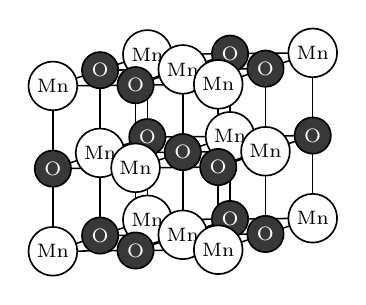
\begin{tikzpicture}[line width=0.8pt,>=Stealth,
  x={(2.1cm,0.02cm)}, y={(1.2cm,0.40cm)}, z={(0cm,2.1cm)}]
\tikzset{bond/.style={line width=0.55pt}}
% ---------- bonds O-Mn (all nearest neighbours inside the cell) ----------
\draw[bond] (0.5,0,0) -- (0,0,0);   \draw[bond] (0.5,0,0) -- (1,0,0);
\draw[bond] (0.5,0,0) -- (0.5,0.5,0); \draw[bond] (0.5,0,0) -- (0.5,0,0.5);
\draw[bond] (0.5,1,0) -- (0,1,0);   \draw[bond] (0.5,1,0) -- (1,1,0);
\draw[bond] (0.5,1,0) -- (0.5,0.5,0); \draw[bond] (0.5,1,0) -- (0.5,1,0.5);
\draw[bond] (0.5,0,1) -- (0,0,1);   \draw[bond] (0.5,0,1) -- (1,0,1);
\draw[bond] (0.5,0,1) -- (0.5,0.5,1); \draw[bond] (0.5,0,1) -- (0.5,0,0.5);
\draw[bond] (0.5,1,1) -- (0,1,1);   \draw[bond] (0.5,1,1) -- (1,1,1);
\draw[bond] (0.5,1,1) -- (0.5,0.5,1); \draw[bond] (0.5,1,1) -- (0.5,1,0.5);
\draw[bond] (0,0.5,0) -- (0,0,0);   \draw[bond] (0,0.5,0) -- (0,1,0);
\draw[bond] (0,0.5,0) -- (0.5,0.5,0); \draw[bond] (0,0.5,0) -- (0,0.5,0.5);
\draw[bond] (1,0.5,0) -- (1,0,0);   \draw[bond] (1,0.5,0) -- (1,1,0);
\draw[bond] (1,0.5,0) -- (0.5,0.5,0); \draw[bond] (1,0.5,0) -- (1,0.5,0.5);
\draw[bond] (0,0.5,1) -- (0,0,1);   \draw[bond] (0,0.5,1) -- (0,1,1);
\draw[bond] (0,0.5,1) -- (0.5,0.5,1); \draw[bond] (0,0.5,1) -- (0,0.5,0.5);
\draw[bond] (1,0.5,1) -- (1,0,1);   \draw[bond] (1,0.5,1) -- (1,1,1);
\draw[bond] (1,0.5,1) -- (0.5,0.5,1); \draw[bond] (1,0.5,1) -- (1,0.5,0.5);
\draw[bond] (0,0,0.5) -- (0,0,0);   \draw[bond] (0,0,0.5) -- (0,0,1);
\draw[bond] (0,0,0.5) -- (0.5,0,0.5); \draw[bond] (0,0,0.5) -- (0,0.5,0.5);
\draw[bond] (1,0,0.5) -- (1,0,0);   \draw[bond] (1,0,0.5) -- (1,0,1);
\draw[bond] (1,0,0.5) -- (0.5,0,0.5); \draw[bond] (1,0,0.5) -- (1,0.5,0.5);
\draw[bond] (0,1,0.5) -- (0,1,0);   \draw[bond] (0,1,0.5) -- (0,1,1);
\draw[bond] (0,1,0.5) -- (0.5,1,0.5); \draw[bond] (0,1,0.5) -- (0,0.5,0.5);
\draw[bond] (1,1,0.5) -- (1,1,0);   \draw[bond] (1,1,0.5) -- (1,1,1);
\draw[bond] (1,1,0.5) -- (0.5,1,0.5); \draw[bond] (1,1,0.5) -- (1,0.5,0.5);
\draw[bond] (0.5,0.5,0.5) -- (0.5,0.5,0); \draw[bond] (0.5,0.5,0.5) -- (0.5,0.5,1);
\draw[bond] (0.5,0.5,0.5) -- (0.5,0,0.5); \draw[bond] (0.5,0.5,0.5) -- (0.5,1,0.5);
\draw[bond] (0.5,0.5,0.5) -- (0,0.5,0.5); \draw[bond] (0.5,0.5,0.5) -- (1,0.5,0.5);
% ---------- atoms, back (y=1) to front (y=0) ----------
\newcommand\mn[3]{\node[circle,draw=black,fill=white,line width=0.6pt,inner sep=1.9pt] at (#1,#2,#3) {\scriptsize Mn};}
\newcommand\ox[3]{\node[circle,draw=black,fill=black!78,text=white,line width=0.6pt,inner sep=1.9pt] at (#1,#2,#3) {\scriptsize O};}
% back layer y = 1
\mn{0}{1}{0} \mn{1}{1}{0} \mn{0}{1}{1} \mn{1}{1}{1} \mn{0.5}{1}{0.5}
\ox{0.5}{1}{0} \ox{0.5}{1}{1} \ox{0}{1}{0.5} \ox{1}{1}{0.5}
% middle layer y = 0.5
\mn{0.5}{0.5}{0} \mn{0.5}{0.5}{1} \mn{0}{0.5}{0.5} \mn{1}{0.5}{0.5}
\ox{0}{0.5}{0} \ox{1}{0.5}{0} \ox{0}{0.5}{1} \ox{1}{0.5}{1} \ox{0.5}{0.5}{0.5}
% front layer y = 0
\mn{0}{0}{0} \mn{1}{0}{0} \mn{0}{0}{1} \mn{1}{0}{1} \mn{0.5}{0}{0.5}
\ox{0.5}{0}{0} \ox{0.5}{0}{1} \ox{0}{0}{0.5} \ox{1}{0}{0.5}
\end{tikzpicture}
\end{document}
